\documentclass[hyperref={pdfpagelabels=true}]{beamer}
\usepackage{lmodern}
\usepackage{graphicx}
\usepackage{tikz}
\usepackage[framemethod=tikz]{mdframed}
\usepackage{ragged2e}

%%%%%%%%%%%%%%%%%%%%%%%%%%%%%%%%%%%%%%%%%%%%%%%%%%%%%%%%%%%%%%%%%%%%%%%%%%%%%%%%%%%%%%%%%%%%%%%%%
%This work is licensed under a Creative Commons Attribution-ShareAlike 4.0 International License.
%
%You are free to:
%
%    Share — copy and redistribute the material in any medium or format
%    Adapt — remix, transform, and build upon the material
%    for any purpose, even commercially.
%
%    The licensor cannot revoke these freedoms as long as you follow the license terms.
%
%Attribution — You must give appropriate credit, provide a link to the license, and indicate if changes were made. You may do so in any reasonable manner, but not in any way that suggests the licensor endorses you or your use.
%
%ShareAlike — If you remix, transform, or build upon the material, you must distribute your contributions under the same license as the original. 
%
%%%%%%%%%%%%%%%%%%%%%%%%%%%%%%%%%%%%%%%%%%%%%%%%%%%%%%%%%%%%%%%%%%%%%%%%%%%%%%%%%%%%%%%%%%%%%%%%%

\newmdenv[tikzsetting={draw=black,fill=white,fill opacity=0.5, line width=0pt},
      backgroundcolor=none,leftmargin=0,rightmargin=0,innertopmargin=4pt]
      {titleBox}

\setbeamertemplate{caption}{\raggedright\insertcaption\par} 
\setbeamerfont{caption}{size=\scriptsize}

\definecolor{dred}{rgb}{0.647059, 0.164706, 0.164706}
\definecolor{dgreen}{rgb}{0., 0.545098, 0.545098}

\setbeamerfont{caption}{size=\tiny}
%\usecolortheme[named=dred]{structure}

%\usetheme{Marburg}
%\usecolortheme{crane}

%\usetheme{AnnArbor}
%\usecolortheme{wolverine}

\usetheme{Warsaw}
\usecolortheme{dolphin}

%\title{Horizontes no Panorama da Ci\^{e}ncia de Dados Espaciais}
\title{Ci\^{e}ncia de Dados Espaciais}
\subtitle{Aonde Vamos?}
\author{Joana Sim\~{o}es} 

\author[shortname]{Joana Sim\~{o}es \inst{1}}
\institute[shortinst]{\inst{1} Eurecat, Centro Tecnol\'{o}gico da Catalunha}

%\date{\today} 
%\titlegraphic{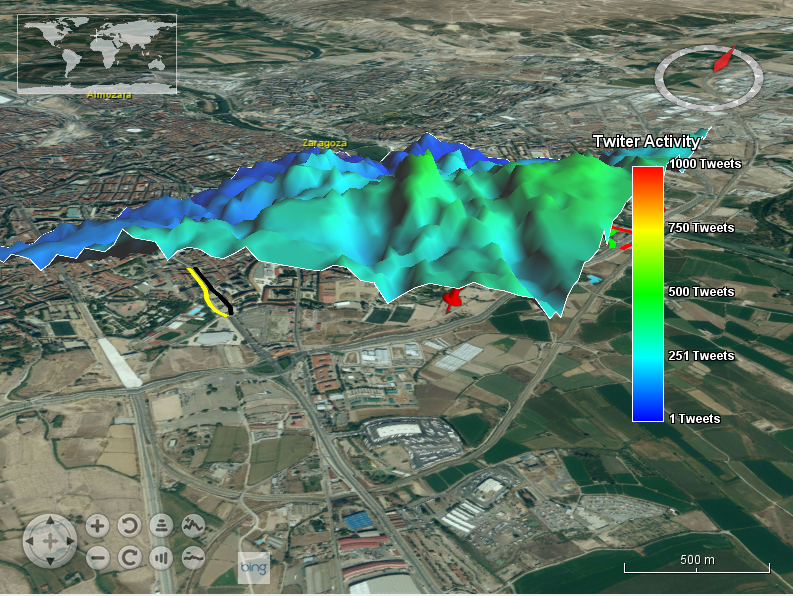
\includegraphics[width=.35\textwidth]{3d2.png}}

\usepackage{listings}

\newcommand{\soooo}{H$_2$SO$_4$}

%fdl stuff
\usepackage{hyperref}
\hypersetup{colorlinks, 
           citecolor=black,
           filecolor=black,
           linkcolor=blue,
           urlcolor=blue,
           bookmarksopen=true,
           pdftex}

\hfuzz = .6pt % avoid black boxes

\lstset{language=SQL}



\begin{document}
\setbeamertemplate{footline}[page number]
\setbeamertemplate{navigation symbols}{}

%\titlepage

{ \usebackgroundtemplate{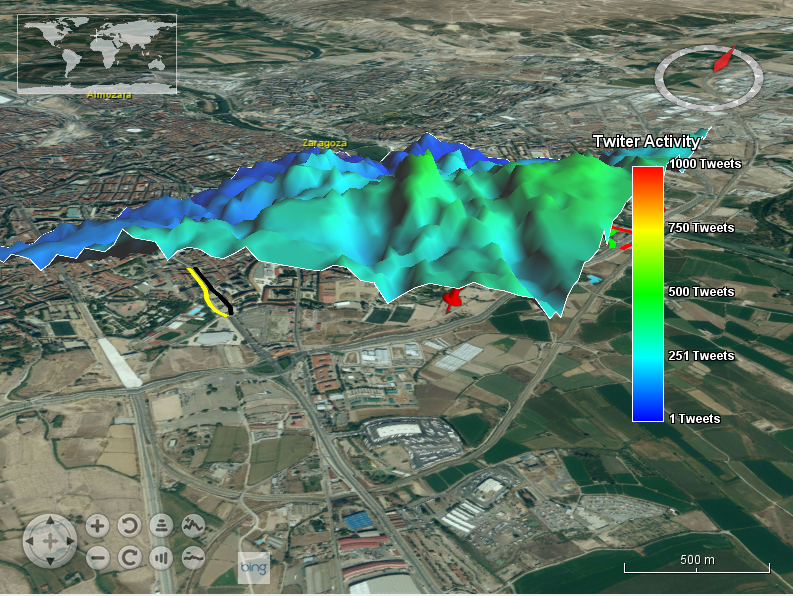
\includegraphics[width=\paperwidth]{3d2.png}} 
\begin{frame}[plain]
    \vspace{10em}
    \begin{titleBox}
        \centering \textbf{Ci\^{e}ncia de Dados Espaciais}\\
        \textbf{Aonde Vamos?}\\  
        \justify
        \small{Joana Sim\~{o}es}\\
        \small{Eurecat, Centro Tecnol\'{o}gico da Catalunha\\
        }
        
    \end{titleBox}

%\frametitle{Frame with nice background} 
%\begin{itemize} \item 1 \item 2 \item 3 \end{itemize}
\end{frame} 
} 
 
%\begin{frame}
%\frametitle{Tabela de Conte\'{u}dos}
%\tableofcontents
%\end{frame}

%TODO: reference list, acentos

\section{Introdu\c{c}\~{a}o} 
\begin{frame}
\frametitle{Cientistas \& Unic\'{o}rnios}
\centering
\tiny{ 
      \begin{itemize}    
       \item<1->\small{``Data Scientist'' is a Data Analyst who lives in California.} 
       \item<1->A data scientist is someone \textit{who is better at statistics than any software engineer and better at software engineering than any statistician.} (Wills, Cloudera)
      \end{itemize}                
}
    \begin{figure}   
         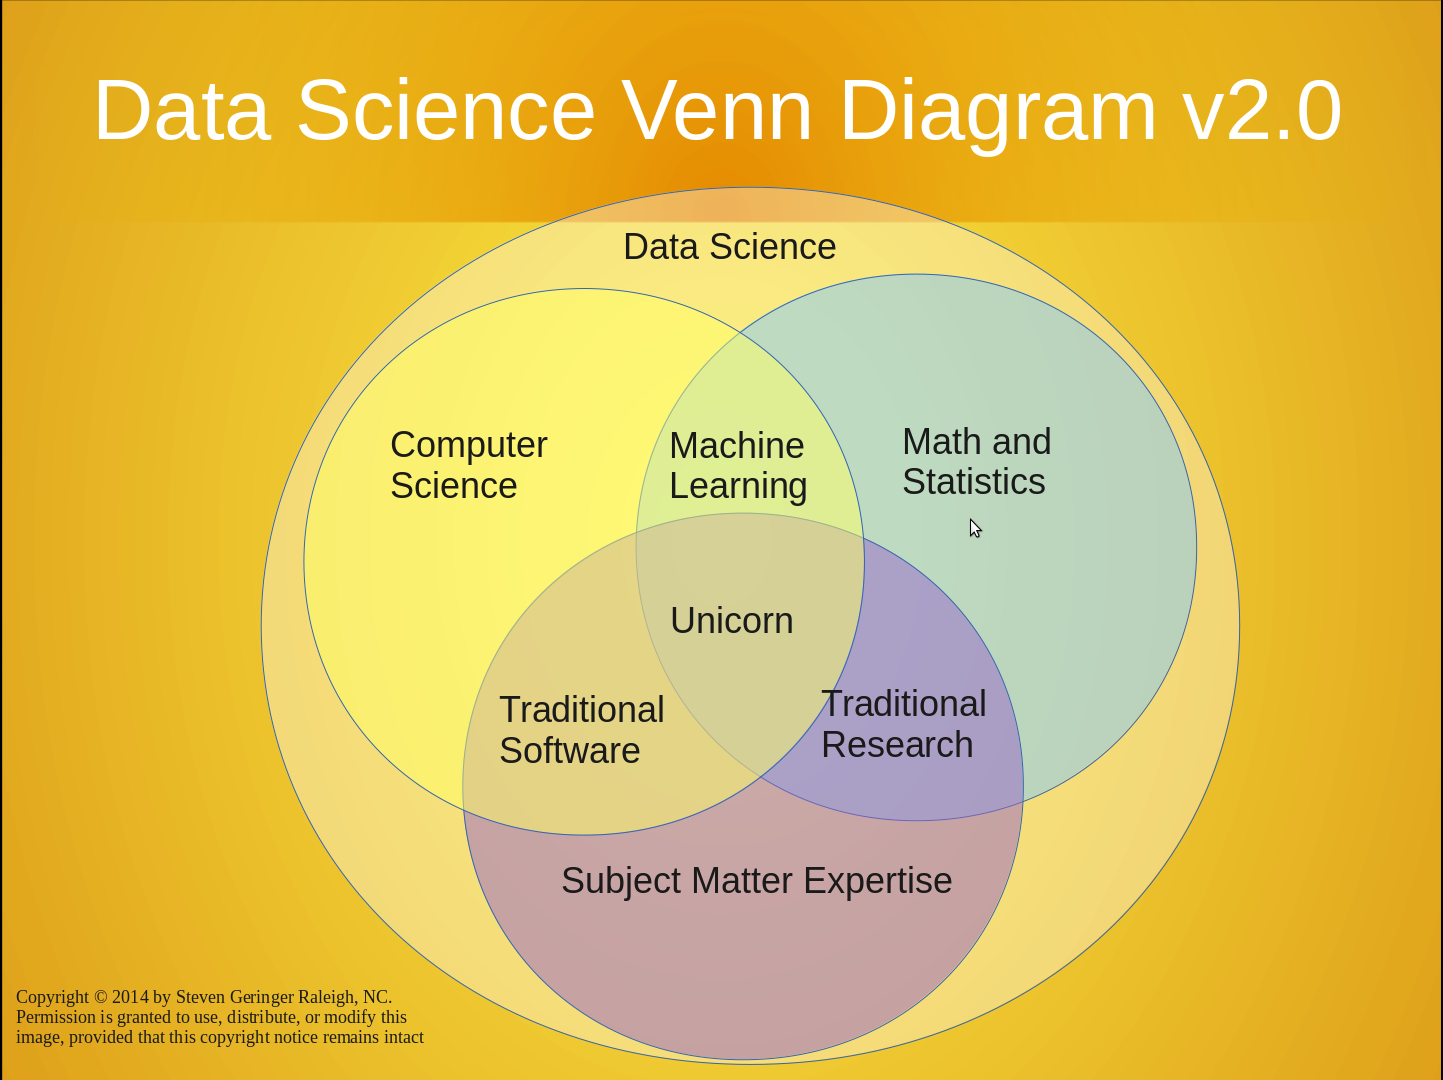
\includegraphics[width=0.7\textwidth]{venn.png}  
          %\caption{Ciencia de dados}
    \end{figure}     


\end{frame}


\begin{frame}
\frametitle{Dados, Informa\c{c}\~{a}o e Conhecimento}

%\small{ 
%      \begin{itemize}    
%        \item<1->Dados sao os factos que descrevem o mundo.%e.g.: temperatura, idade, numero de degraus da escada de casa
%        \item<1->A informacao surge quando transformamos esses valores em algo relevante.%Pode ajudar-nos a tomar decisoes informadas
%        \item<1->Conhecimento implica uma generalizacao dos dados e da informacao, de forma a criar regras.%'Nteste processo podemos simular a inteligencia humana, atraves de modelos analiticos
%      \end{itemize}                
%}

    \begin{figure}   
         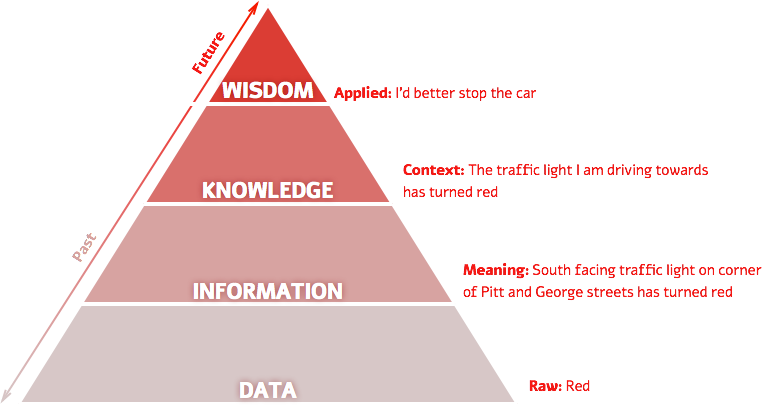
\includegraphics[width=0.8\textwidth]{pyramid2.png}   
    \end{figure}     


\end{frame}

\begin{frame}
\frametitle{Algo \textit{espacial}...}

Lei de Tobler:\\
\textit{Everything is related to everything else, but near things are more related to each other.}%First Law of Geography

\begin{figure}
	\includegraphics[width=0.7\textwidth]<1>{cruise.png}       
	\includegraphics[width=0.7\textwidth]<2>{schools.png}	
        \caption{\only<1>{Heatmap de Tweets perto de um Cruzeiro (Eurecat, unpublished).}\only<2>{Buffers de acidentes \`{a} volta das escolas (Eurecat, unpublished).}}           	
\end{figure}
\end{frame}

%\begin{frame}
%\frametitle{Problemas Fundamentais}

%Longley \textit{ET AL} (2005):
%\small{ 
%      \begin{itemize} 
%      \item<2->O comportamento espacial actual, muitas vezes reflecte padroes passados.%necessidade de estudar series temporais
%        \item<3->A explicacao no tempo apenas necessita de olhar para o passado, mas a explicacao no espaco necessita de olhar em todas as direccoes simultaneamente.%A autocorrelacao temporal tem uma dimensao, enquanto que a autocorrelacao espacial tem duas ou tres dimensoes
%        \item<4->Embora alguns fenomenos espaciais variem de forma gradual atraves do espaco, outros podem exibir uma extrema irregularidade.%break Toblers Law. Por exemplo acidentes de trafico
%        \item<5->Embora a autocorrelacao espacial nos ajude a construir representacoes, ela pode frustrar os nossos esforcos de predicao.% patterns of spatial autocorrelation in one variable, would be likely mirrored on others, but that does not imply any causality.
%      \end{itemize}                
%}

%\end{frame}


\section{Tend\^{e}ncias} 
\begin{frame}
\frametitle{Onde Vamos?}

    \begin{figure}   
         
\includegraphics[width=0.7\textwidth]{fortune-teller.png}   
    \end{figure}     

\end{frame}


\begin{frame}
\frametitle{(Algumas) Tend\^{e}ncias}

    \begin{figure}   
         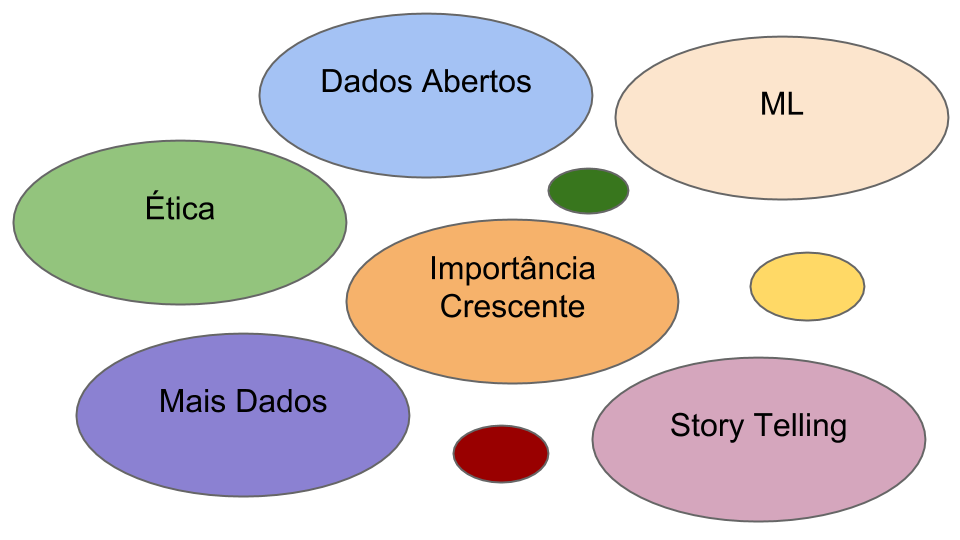
\includegraphics[width=\textwidth]{trends.png}   
    \end{figure}     
    
\end{frame}


\begin{frame}
\frametitle{Import\^{a}ncia Crescente}

      %\begin{itemize}    %ubiquidade da ciencia de dados, e nao so reservada a investigacao
       % \item<1->A ciencia de dados ganha torna-se cada vez mais importante, a medida que entra em novos campos.%personal health eHealth
        %\item<2->A Geografia tambem benefia desse impulso, a medida que o publico em geral toma consciencia de que a maior parte das coisas, acontecem num lugar.
      %\end{itemize}                
      
    \begin{figure}   
         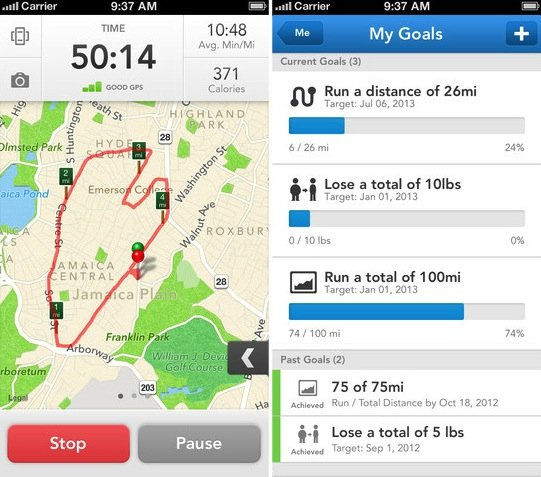
\includegraphics[width=0.3\textwidth]{runkeeper.jpg}
         \caption{Runkeeper: fitness track app \url{https://runkeeper.com/}}
    \end{figure} 
    
    \begin{figure}  
	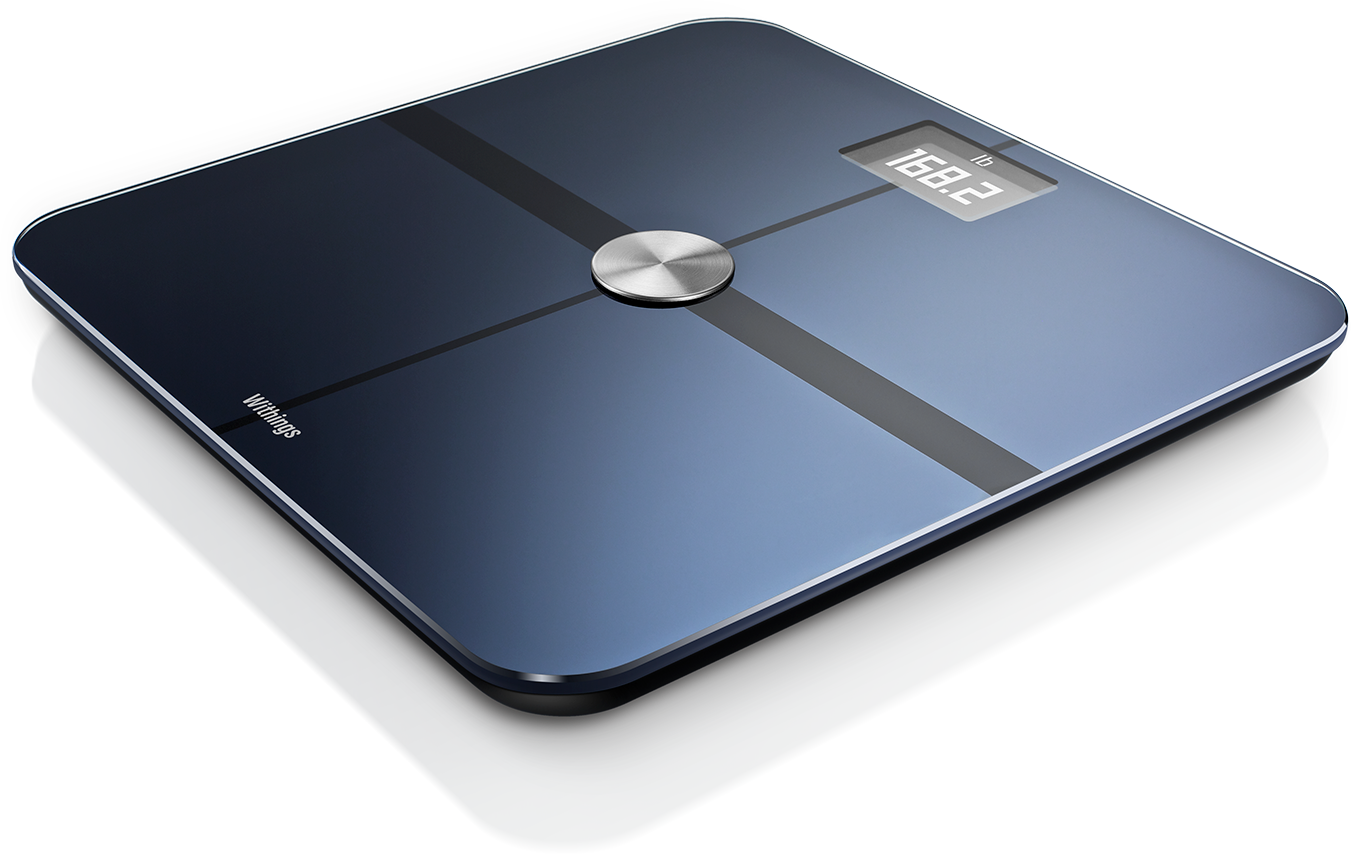
\includegraphics[width=0.3\textwidth]{scale.png}
	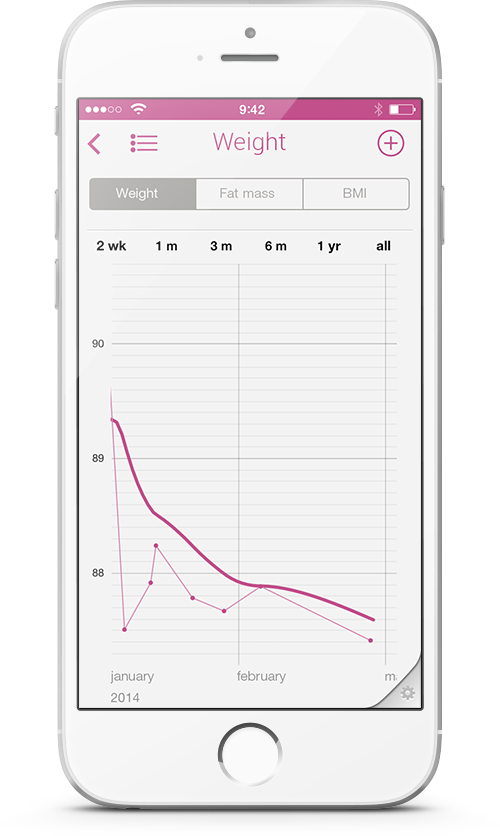
\includegraphics[width=0.1\textwidth]{app.png}
         \caption{\textit{Whitings}: balanca ``inteligente'' \url{http://www2.withings.com/eu/en}}		
       \end{figure}  
    
    

\end{frame}

%\begin{frame}
%\frametitle{Import\^{a}ncia Crescente (cont.)}

%      \begin{itemize}
%        \item<1->\textit{Whitings} e uma balanca ``inteligente''.
%        \item<2->Recolhe medicoes corporais precisas: peso, massa gorda e batimentos cardiacos.
%        \item<3->Uma app analisa estes dados, mostra tendencias e permite gerar planos e monitorizar metas.%por exemplo para perder peso 
%      \end{itemize}                
      
%\end{frame}

%Outro exemplo: seguranca pessoal de idosos?



\begin{frame}
\frametitle{Mais Dados}
%Automaticos

      %\begin{itemize}
       % \item<1->Existe uma explosao na quantidade de dados gerados por sensores (IoT, IoE).
        %\item<2->Gracas a tecnologias de posicionamento mais baratas e generalizadas (e.g.: receptores de GPS), uma proporcao grande destes dados esta georeferenciada.
      %\end{itemize}                
    \begin{figure}        
	\includegraphics[width=\textwidth]<1>{iot2.png}%37 billions devices
	%\includegraphics[width=0.6\textwidth]<2>{drones.png}
        %\caption{\only<1>{Infografia baseada en dados da Cisco \url{http://www.i-scoop.eu/internet-of-things/}}\only<2>{UAV drones, utilizados para levantamentos geodesicos (Wallace ET AL, 2012)}}   %http://www.mdpi.com/2072-4292/4/6/1519      
        \caption{\only<1>{Infografia baseada en dados da Cisco \url{http://www.i-scoop.eu/internet-of-things/}}}
    \end{figure}  


\end{frame}

%\begin{frame}
%\frametitle{Mais Dados (cont.)}
%Automaticos
 %     \begin{itemize}
  %      \item<1->LIDAR: mede propriedades da luz reflectida de modo a obter a distancia ou outra informacao a respeito um determinado objecto distante.
   %     \item<2->O UAV LIDAR aplica esta tecnica a partir de um drone.%permite fazer levantamentos geodesicos muito acurados, e com baixo custo; funciona em sitios com nuvens, ou em tuneis, onde o sinal de GPS 'e limitado
        %TODO: arranjar um exemplo
        %e airborne ops run for 7 days only and acquired billions of laser points and thousands of air photo on project area blocks encompassing approximately 29,000 Ha - See more at: http://blog.lidarnews.com/uavs-set-to-revolutionize-archaeological-mapping/#sthash.0aofVAFp.dpuf
    %  \end{itemize}                
%tempos excitantes para a arqueolologia
    %\begin{figure}   
     %    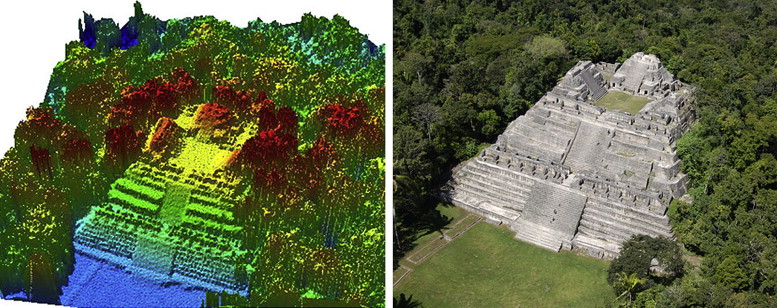
\includegraphics[width=0.8\textwidth]{lidar.jpg} %choque com um aviao  
    %\end{figure} 
            
%\end{frame}

%\begin{frame}
%\frametitle{E Ainda Mais Dados}
%Nao-automaticos
%      \begin{itemize}
%        \item<1->Existe uma explosao na quantidade de UGC.
%        \item<1->voluntario: citizens as sensors e VGI (p.e: OSM).
%        \item<1->Nao-voluntario (?): gerados nas redes sociais (p.e: Twitter).        
%      \end{itemize}                

%    \begin{columns}
%    \begin{column}{0.5\textwidth}
%        \begin{figure}  
%            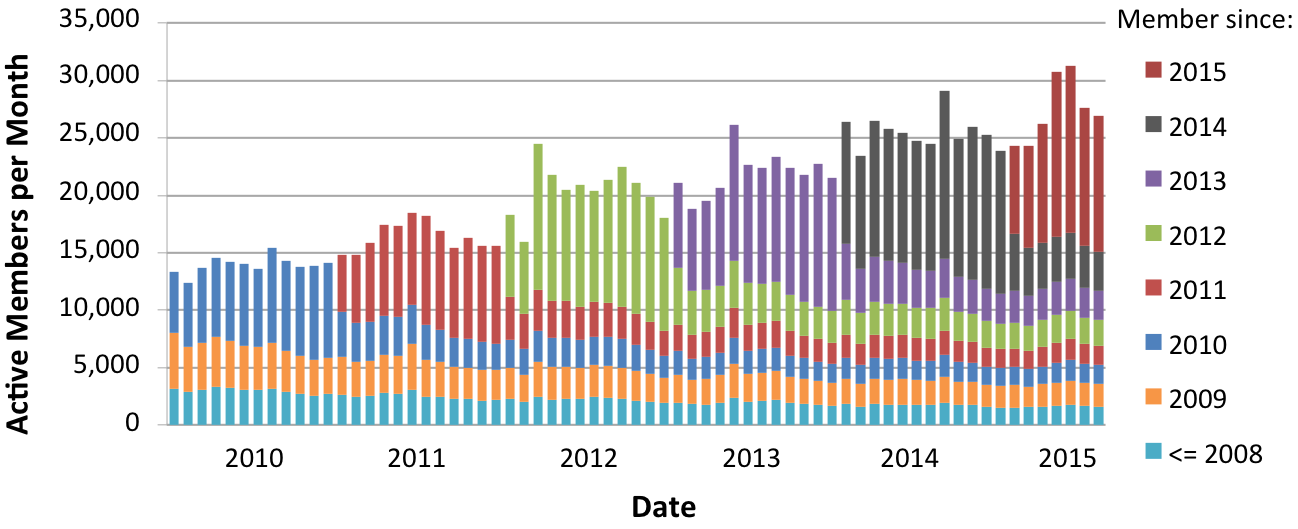
\includegraphics[width=0.7\textwidth]{osm_members.png}\\
%            \tiny{Evolucao do numero de membros do OSM.}
%        \end{figure}             
%    \end{column}
%    \begin{column}{0.5\textwidth}
%        \begin{figure}  
%            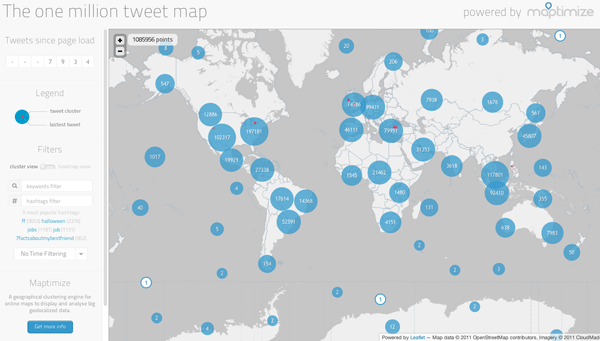
\includegraphics[width=0.7\textwidth]{twittermap.png}\\
%            \tiny{Mapa com a localizacao do ultimo milhao de Tweets.}
%        \end{figure}  
%    \end{column}  
%    \end{columns} 

%\end{frame}


\begin{frame}
\frametitle{E Ainda Mais Dados}

 %     \begin{itemize}
        %\item<1->Com a chegada de cruzeiros ao Porto de Barcelona, ha uma explosao no numero de Tweets.
 %       \item<2->Um metodo de deteccao de origem, permite diferenciar os Tweets gerados por locais dos gerados por estrangeiros.
 %       \item<3->Podemos observar que ha um acrescimo no numero de Tweets gerados por estrangeiros, apos a chegada dos cruzeiros ao Porto de Barcelona.
        %\item<1->Com base nesta classificacao, podemos observar que estes dois grupos se distribuem diferentemente pela cidade.        
 %     \end{itemize}                

        \begin{figure}  
            
\includegraphics[width=0.2\textwidth]{twitter.jpg}
        \end{figure}  

 
        \begin{figure}  
            \includegraphics[width=0.5\textwidth]<1>{normal_vs_foreign_CapSetmanaCreuers.png}
            \includegraphics[width=0.5\textwidth]<2>{barriosForeignUsersCapSetmanaCreuers_cnt.png}
            \caption{\only<1>{Clusters de Tweets enviados por locais e estrangeiros (Eurecat, unpublished).}\only<2>{Distribui\c{c}\~{a}o de densidades de Tweets enviados por estrangeiros (Eurecat, unpublished).}}
        \end{figure}  

\end{frame}


\begin{frame}
\frametitle{``Arqueologia'' de Dados}

      %\begin{itemize}
       % \item<1->Existe uma necessidade crescente de ``recuperar'' fontes de dados de legacy (por exemplo em formato analogico)
        %\item<2->Embora isto implique um desafio tecnologico, muitas vezes estes conjuntos de dados sao extremamente valiosos.%explicar porque
      %\end{itemize}                
    \begin{figure}   
         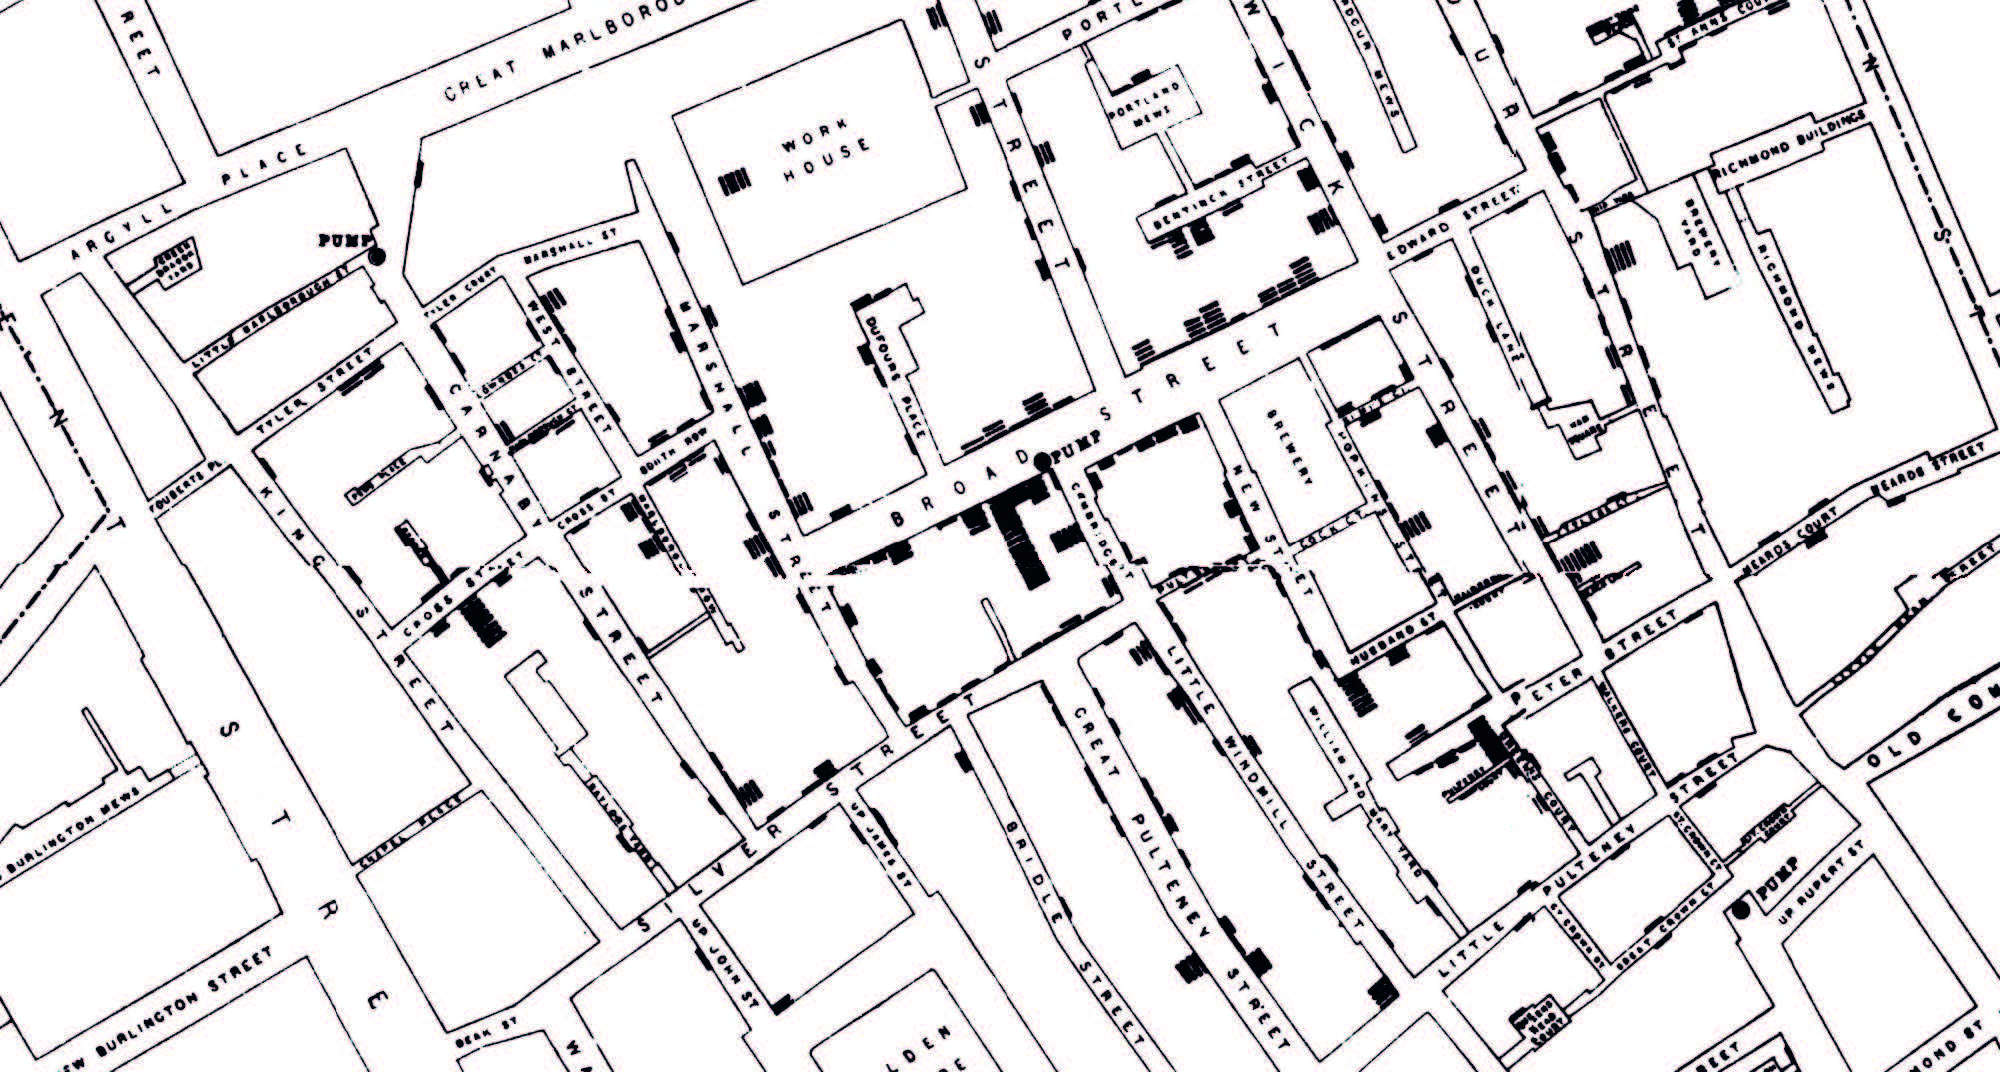
\includegraphics[width=0.6\textwidth]{snow.jpg}\\
         \tiny{Mapa de casos de c\'{o}lera em Londres, produzido por John Snow (1864).}
    \end{figure} 

    \begin{figure}   
         \includegraphics[width=\textwidth]<2>{fao.png}
         \caption{\only<2>{Descodifica\c{c}\~{a}o de metadados atrav\'{e}s da estrutura de direct\'{o}rios (Institute of Marine Research, unpublished).}}
    \end{figure} 
    
\end{frame}

%\begin{frame}
%\frametitle{``Arqueologia'' de Dados (cont.)}

%      \begin{itemize}      
%        \item<1->Dados de informacao de pescas (biomassas), foram guardados sem metadados.
%        \item<2->Para capturar estes dados, foi necessario efectuar cruzeiros com um custo elevadissimo.%valor em $$$
%        \item<3->A informacao capturada e irrepetivel.%valor em unicidade        
%        \item<4->Os metadados estao encodificados na path do ficheiro (i.e.: timestamp, nome do cruzeiro).%foi necessario criar uma aplicacao que navegue e interprete as paths no disco, e as associe aos ficheiros
        %A aplicacao tem de ser monitorizada por um operador
%      \end{itemize}                
%    \begin{figure}   
%         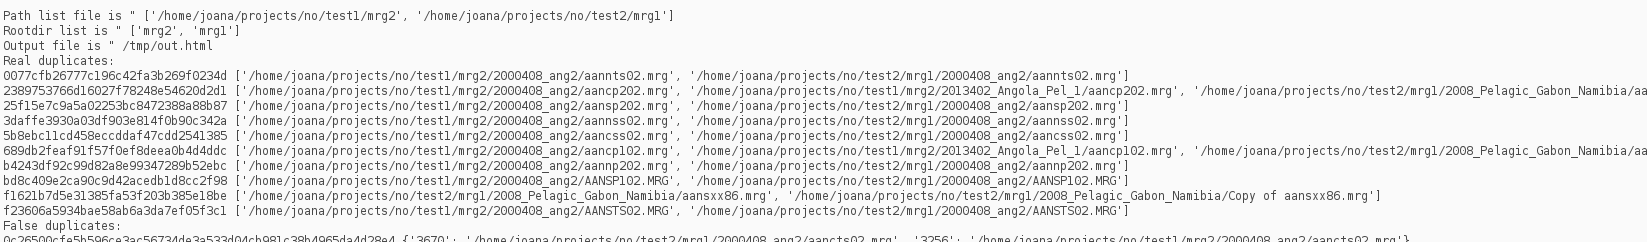
\includegraphics[width=0.8\textwidth]{fao.png}
%   \end{figure} 
%\end{frame}

\begin{frame}
\frametitle{Tecnologias de \textit{Big Data}}

      %\begin{itemize}      
       % \item<1->3 Vs.
       % \item<2->Computacao em ambiente Cloud, NoSQL, Processamento em tempo-real ,Linked Data.%web semantica
       % \item<4->Big Spatial Data.
      %\end{itemize}                
    %\begin{figure}   
     %    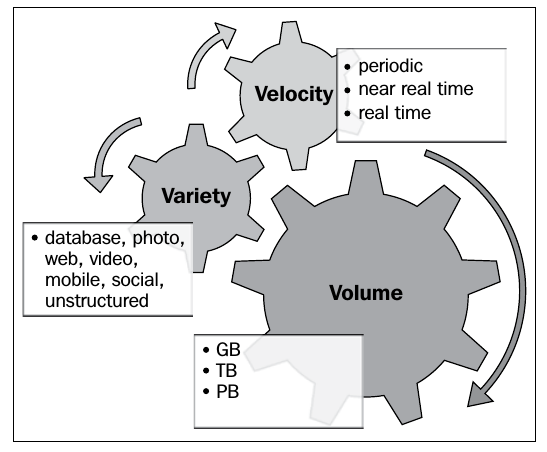
\includegraphics[width=0.5\textwidth]{3vs.png}
    %\end{figure} 
    
        \begin{figure}  
            \includegraphics[width=0.7\textwidth]<1>{3vs.png}
            \includegraphics[width=0.7\textwidth]<2>{general1.png}
            \caption{\only<1>{Os 3 Vs de Big Data (Cuesta, H., 2013).}\only<2>{Benchmarking de bases de dados espaciais na cloud (Simoes, 2015).}}%Practical data analysis
        \end{figure}  

\end{frame}


%\frametitle{Tecnologias de \textit{Big Data} (cont.)}
%\begin{frame}
%Desenvolvimento de tecnologias espaciais escalaveis e distribuidas.
%      \begin{itemize}      
%        \item<2->Suporte espacial ainda limitado.%implementado em poucas tecnologias e com limitacoes
%        \item<3->Necessidade crescente de saber em que situacoes utilizar cada tecnologia.%trade offs nem sempre sao claros: benchmarking
%      \end{itemize}                
%    \begin{figure}   
%         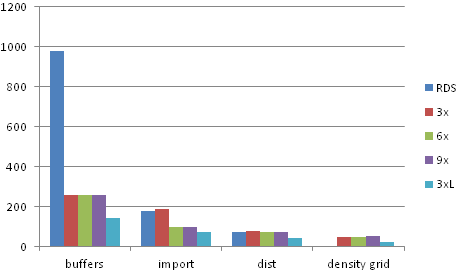
\includegraphics[width=0.7\textwidth]{general1.png}\\
%         \tiny{Benchmarking de bases de dados espaciais na cloud;.}%relacionais vs cluster         
%    \end{figure} 
%\end{frame}

\begin{frame}
\frametitle{Uso Cada vez Mais Generalizado de \textit{ML}}
%A disponibilidade crescente de dados e os progressos computacionais vao impulsionar o uso de Machine Learning.
%      \begin{itemize}      
%        \item<2->Ascendencia algoritmos computacionalmente intensivos (p.e.: Deep Learning)%
%        \item<3->Modelos Ensemble.%Grid search for parameters
%        \item<4->Modelos espaciais.%Mts dimensoes
%        \item<5->Descriptivo $\rightarrow$ Predictivo
%      \end{itemize}                
    \begin{figure}   
         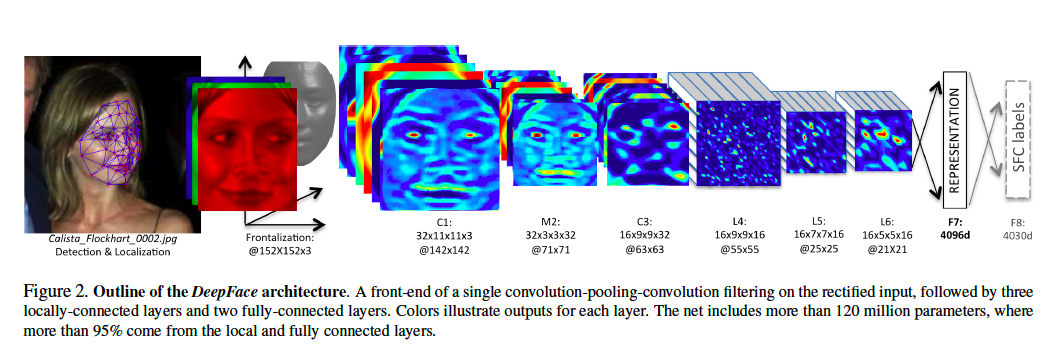
\includegraphics[width=0.6\textwidth]{deep.png}
         \caption{Arquitectura de uma red de Deep Learning para reconhecimento facial \url{https://gigaom.com/2015/03/06/how-paypal-uses-deep-learning-and-detective-work-to-fight-fraud/}.}%Facebook
    \end{figure} 
    
    \begin{figure}   
        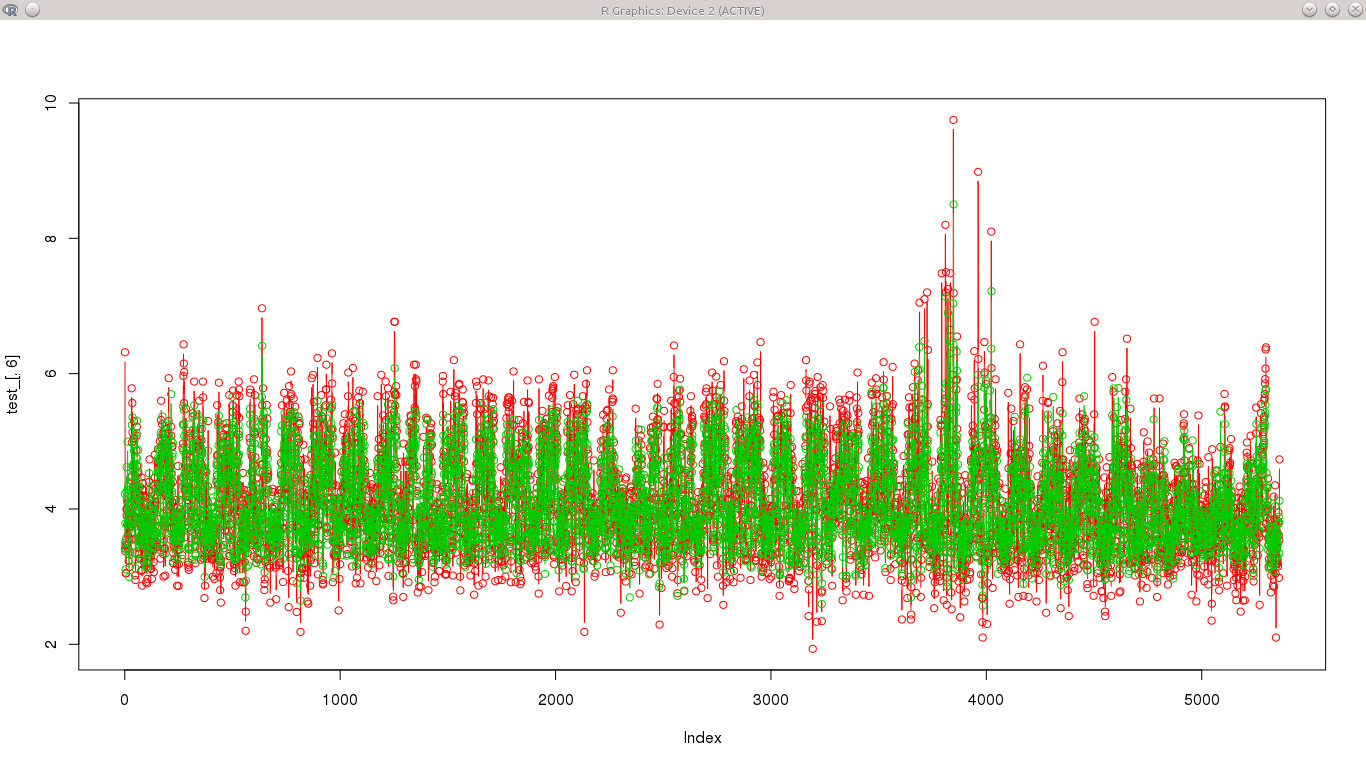
\includegraphics[width=0.5\textwidth]{prediction.png}
        \caption{Tempos de viagem na cidade de Barcelona: ajuste entre as previs\~{o}es SVM (verde) e os valores observados (vermelho) (Eurecat, unpublished).}
    \end{figure} 
    
\end{frame}

%\begin{frame}
%\frametitle{Uso Cada vez Mais Generalizado de \textit{ML} (cont.)}

%    Trafico e um dominio onde tradicionalmente se utilizam modelos de micro-simulacao.
%      \begin{itemize}         
%        \item<2->Foram aplicados modelos de ML para prever os tempos de viagem na cidade de Barcelona.
%        \item<3->Os modelos foram treinados e validados com um ano de dados.
%        \item<4->A ANN foi descartada a favor de uma SVM.
%       \end{itemize}            
          

%\end{frame}


\begin{frame}
\frametitle{Jornalismo de Dados \& \textit{Story Telling}}
 %“those who tell stories rule society.” 
      %%\begin{itemize}         
        %\item<1->Os dados quantitativos teem um papel cada vez mais valorizado na producao e distribuicao de informacao.
        %\item<2->Existe uma necessidade crescente de apresentar ``historias'' de dados a uma audiencia mais vasta (infografia).
        %\item<3->As visualizacoes (incluindo mapas) podem ser uma ferramenta valiosa.
       %\end{itemize}            
          
        %\begin{figure}   
         %   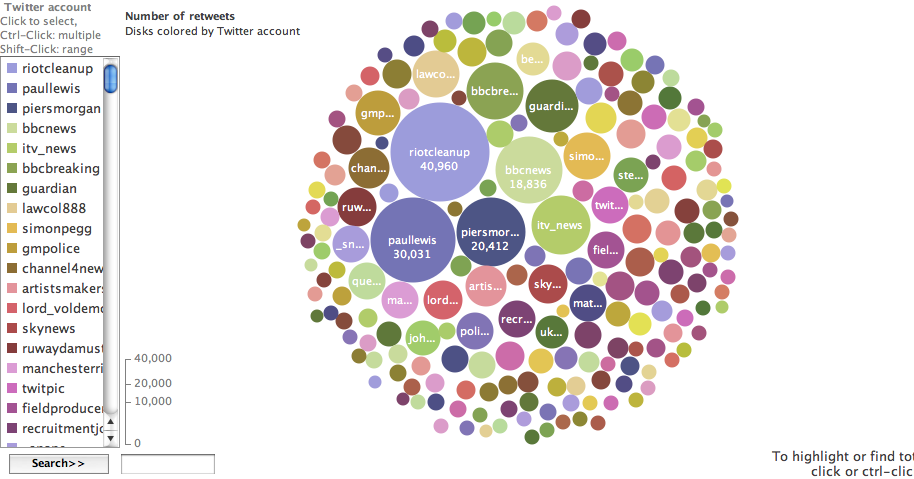
\includegraphics[width=0.6\textwidth]{guardian.png}\\
         %\tiny{Visualizacao de retweets de um rumor, por Twitter account}%Guardian: put source            
        %\end{figure} 
        
        \begin{figure}  
            \includegraphics[width=0.8\textwidth]<1>{guardian.png}
            \includegraphics[width=\textwidth]<2>{dashboard.png}
            \caption{\only<1>{How riot rumours spread on Twitter (Guardian Interactive team, 2011).}\only<2>{Dashboard sobre acidentes graves e mortais na cidade de Barcelona (Eurecat, unpublished).}}%Practical data analysis            
        \end{figure} 
        
\end{frame}

%\begin{frame}
%\frametitle{Jornalismo de Dados \& \textit{Story Telling} (cont.)}

%    \small{
%     As dashboard dao a possibilidade de visualizar os dados de forma dinamica, e em tempo real.
%      \begin{itemize}         
        %\item<1->Sao uma ferramenta cada vez mais utilizada para contar historias ``guiadas'' pelos dados.
%        \item<2->Uma dashboard foi desenvolvida para transmitir os insights sobre acidentes graves e mortais na cidade de Barcelona.
        %\item<3->Uma serie de widgets (graficos, mapas, metricas) descrevem os dados de acidentes.
%        \item<3->A stack utilizada (ELK) permite uma actualizacao em tempo real.%ELK
%       \end{itemize}            
%      }    

%\end{frame}



\begin{frame}
\frametitle{Mais (e Melhores) Dados Abertos}

      %\begin{itemize}         
       % \item<1->``Revolucao'' dos dados abertos.%Seguindo a ``revolucao'' do Software aberto e dos standards abertos
       % \item<2->Cada vez mais instituicoes sao ``pressionadas'' para abrir os seus dados.
       % \item<3->Qualidade dos dados.%problema a abordar: ha vontade, mas n ha dinheiro. mas necessitamos de dados a serio, e nao so formalmente
       %\end{itemize}            
          
        %\begin{figure}   
         %   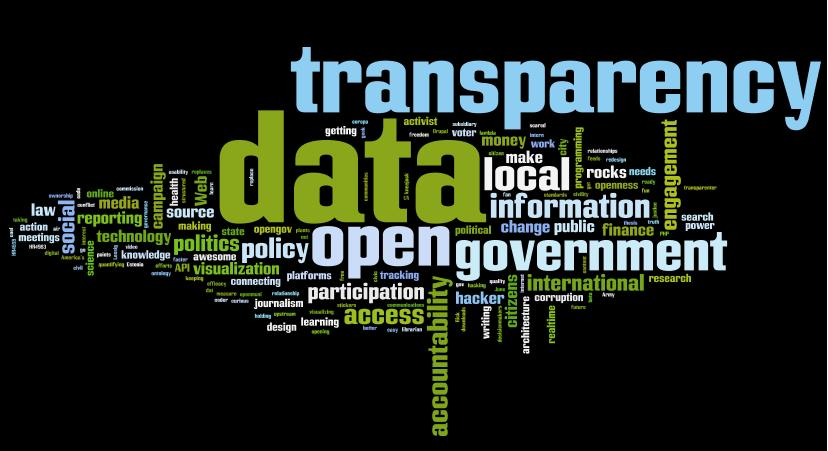
\includegraphics[width=0.6\textwidth]{woordle.jpeg}\\
         %\tiny{Visualizacao de retweets de um rumor, por Twitter account}%Guardian: put source            
        %\end{figure}
        
       %\begin{figure}   
        %    
\includegraphics[width=0.1\textwidth]{od.jpeg}\\%                
            %\tiny{Sismografo da Catalunya @OpenGovCat \url{http://opengov.cat/en/}}         
        %\end{figure} 
        
       \begin{figure}   
            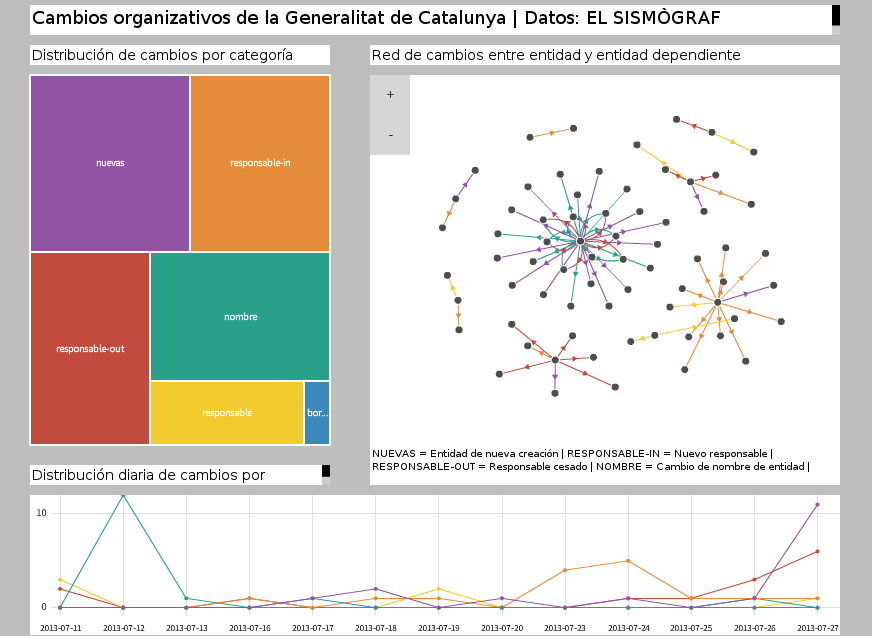
\includegraphics[width=0.7\textwidth]{sism.png}
            %\caption{Sism\'{o}grafo da Catalunya, @OpenGovCat \url{http://opengov.cat/en/}}
            \caption{Sism\'{o}grafo da Catalunya, @OpenGovCat (OpenGov, 2015)}         
        \end{figure} 
 
\end{frame}

%\begin{frame}
%\frametitle{Mais e Melhores Dados Abertos (cont.)}

%    \small{
    %Dados Abertos Publicos: Manter a informacao actualizada = transparencia.
%    \begin{itemize}
%        \item<2->2013: ficheiro actualizado varias vezes por semana com as 8191 entidades que compoem a estrutura do governo e Adminstracao Publica Catala.
%        \item<3->Sismografo da Catalunya @OpenGovCat: permite visualizar estes dados.
%        \begin{itemize}%Que aconteceu no departamento de Agricultura num dia cinzento de Janeiro (2014), quando         
%            \item<4->\textit{Porque foram criadas 32 entidades novas e 57 entidades ficaram subitamente sem responsavel?}
%        \end{itemize}                    
        %\item<5->   Depois de mudar o formato dos dados, em Marco de 2015 a Generalidade deixou de publicar os dados.%numa altura em que ha mts mudancas (pre-eleitoral)        
%    \end{itemize}                      
%        }
    
%\end{frame}


\begin{frame}
\frametitle{\'{E}tica}
%What do we gain by protecting privacy?
%How about democracy?  Heterogeneity?  Dignity?  (Onsrud, 2005)
%Privacy is the basis of democracy 

    %\begin{itemize}
     %   \item<2->As pessoas estao cada vez mais preocupadas com o uso dos seus dados pessoais, o que esta reflectido em leis de privacidade.
      %  \item<3->Devido a sua natureza, os dados de localizacao sao particularmente sensiveis.
       % \item<4->Existe uma necessidade de desenvolver metodos que abordem estas preocupacoes.
    %\end{itemize}                      
    
     %   \begin{figure}   
      %      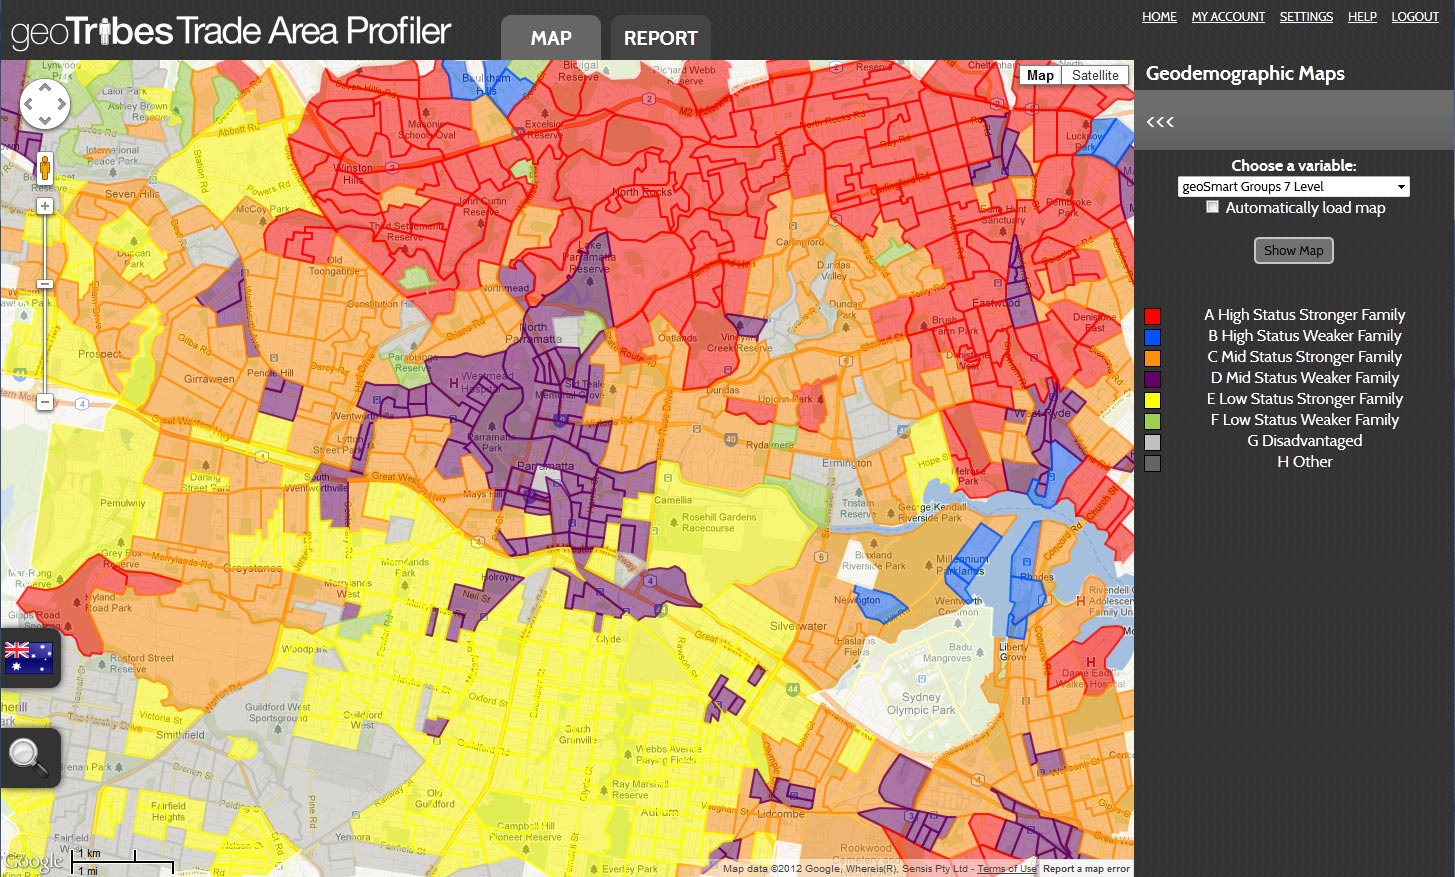
\includegraphics[width=0.4\textwidth]{geodemographics.jpg}\\
       %     \tiny{Os mapas de geodemografia suscitam algumas questoes de privacidade.}%www.rdaresearch.com/blog/page/5/#
        %\end{figure} 
        Ofusca\c{c}\~{a}o espacial (Genovese, A., 2012):
        \begin{itemize}
            \item<2->Annonimity set
            \item<3->MSV        
        \end{itemize}

        \begin{figure}  
            \includegraphics[width=0.5\textwidth]<4>{raw_points.png}
            \includegraphics[width=0.5\textwidth]<5>{ofuscated.png}
            \caption{\only<4>{Pontos originais (Eurecat, unpublished).}\only<5>{Pontos ofuscados (Eurecat, unpublished).}}
        \end{figure}  
        
\end{frame}

%\begin{frame}
%\frametitle{\'{E}tica (cont.)}
%\tiny{
%    \begin{itemize}
        %\item<1->Obfuscacao espacial: altera, substitui ou generaliza a localizacao dos utilizadores, por forma a esconder a sua localizacao real.
        %\item<3->Maximizar a qualidade da informacao, para um grau minimo de anominidade
        %\item<4->Annonimity set: conjunto de individuos que ofusca o individuo.%2: informacao dissociada
        %\item<5->MSV: numero minimo de individuos que aceitamos no grupo.%2: informacao dissociada  
%        \item<6->Transformar os pontos originais (raw points) numa quadricula de densidades, respeitando o MSV.%Quadtree
%    \end{itemize}                      
%}    
%        \begin{figure}   
%            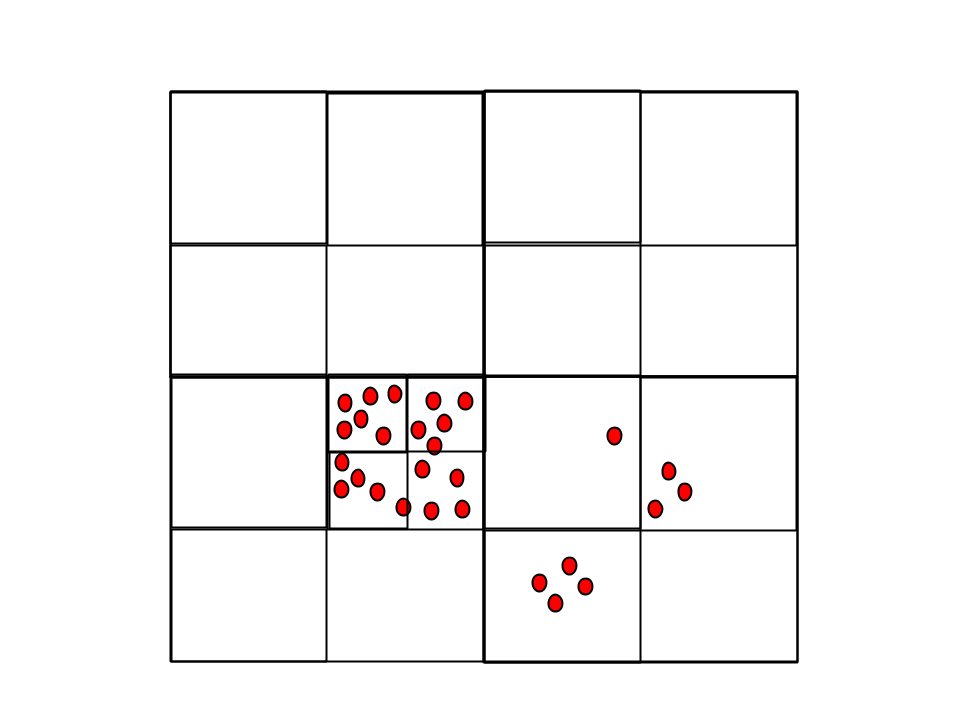
\includegraphics[width=0.4\textwidth]{raw_points.png}
%            \tiny{Raw points vs}
%            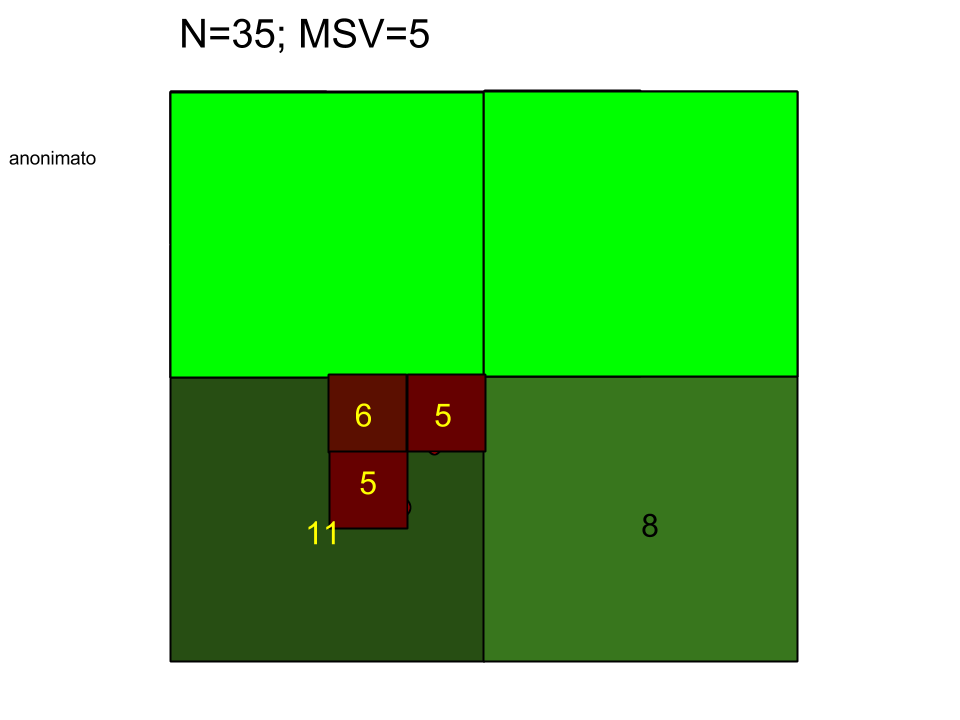
\includegraphics[width=0.4\textwidth]{ofuscated.png}\\
%            \tiny{Ofuscated points.}            
%        \end{figure} 

%\end{frame}


\section{Considera\c{c}\~{o}es Finais} 

\begin{frame}
\frametitle{SIG Open-Source?}

        \begin{figure}   
            
\includegraphics[width=0.8\textwidth]{tux.png}
        \end{figure} 

\end{frame}



\begin{frame}
\frametitle{Import\^{a}ncia destas Tend\^{e}ncias para o FOSS4G}

    Mais aplica\c{c}\~{o}es + maior quantidades de dados = maior comunidade\\%pressao no desenvolvimento
    \begin{itemize}
    
    %Em que areas pode o FOSS4G contribuir para o desenvolvimento da ciencia espacial de dados?
        \item<2->Infra estruturas colaborativas de dados.%OSM, Ushahidi
        \item<2->Bibliotecas de ML com capacidades espaciais.%QGIS, R: point pattern analysis, GWR
        \item<2->Visualiza\c{c}\~{a}o (interactiva) de dados espaciais (3D).%webmapping, virtual globes
        \item<2->Infra estrutura e processamento de Big Spatial Data.
        \item<2->\'{E}tica e privacidade.%O software aberto garante que nao existam backdoors ou codigo malicioso
    \end{itemize}                      

    \centering
        \begin{figure}   
            
\includegraphics[height=1.5cm]{ushahidi.png}        
            
\includegraphics[height=1.5cm]{R.png}
            
\includegraphics[height=1.5cm]{qgis.png}
            
\includegraphics[height=1.5cm]{cartodb.jpg}
            
\includegraphics[height=1.5cm]{nasa.jpg}            
            
\includegraphics[height=1.5cm]{GIS4Hadoop.png}
        \end{figure} 
        
    
\end{frame}


\begin{frame}
\frametitle{Obrigada pela vossa Aten\c{c}\~{a}o}
    Esta apresenta\c{c}\~{a}o encontra-se dispon\'{i}vel em: \centering{\\ \url{http://tinyurl.com/nfbrhvl}\\}
    \begin{figure}   
      
\includegraphics[width=0.5\textwidth]{cat.jpg}      
    \end{figure}   
    
\end{frame}

\begin{frame}
\frametitle{Refer\^{e}ncias}
\tiny{
    \begin{itemize}
    \item Simoes, J., 2015. \textit{Visualizing Geolocated Tweets: A Spatial Data Mining Approach}. Presentation at the 4th Data beers BCN, in Barcelona. Available at: \url{https://github.com/doublebyte1/data_beers/blob/master/data_beers.pdf}
    \item Johnson, S., 2006. The Ghost Map: The Story of London's Most Terrifying Epidemic \textemdash and How it Changed Science, Cities and the Modern World. Riverhead Books. ISBN 1-59448-925-4
    \item Cuesta, H., 2013. Practical Data Analysis. PACKT Publishing. 
    \item Simoes, J., Gim\'{e}nez, R., Planagum\`{a}, M., 2015. \textit{Big Data y Bases de Datos Espaciales: una an\'{a}lisis comparativo}. Presentaci\'{on} en las 9as Jornadas SIG Libre, Girona.
    \item Guardian Interactive team, 2011. \textit{Behind the rumours: how we built our Twitter riots interactive}. Available at: \url{http://www.theguardian.com/news/datablog/2011/dec/08/twitter-riots-interactive}
    \item OpenGov, 2015.\textit{The seismograph's oddyssey and transparency for show}. Available at: \url{http://opengov.cat/en/2015/08/the-seismographs-oddyssey-and-transparency-for-show/}
    \item Genovese, A. 2012. Obfuscation-based techniques for privacy protection in location-based systems: a comparison of recent methods. Dissertation presented for the degree of Doctor in Computer Science, in the Universita Degli Studio di Milano.
    \end{itemize}
}
\end{frame}


\end{document}


